\documentclass{scrartcl}  % scrartcl of scrreprt
% Include all project wide packages here.
\usepackage{fullpage}
\usepackage{polyglossia}
\setmainlanguage{dutch}
\usepackage{csquotes}
\usepackage{graphicx}
\usepackage{epstopdf}
\usepackage{pdfpages}
\usepackage{caption}
\usepackage[list=true]{subcaption}
\usepackage{float}
%\usepackage{mathtools}
\usepackage{standalone}
\usepackage{import}
\usepackage{tocloft}
\usepackage{wrapfig}
\usepackage{authblk}
\usepackage{array}
\usepackage{booktabs}
\usepackage[toc,page,title,titletoc]{appendix}
\usepackage{xunicode}
\usepackage{amsmath}
\usepackage{fontspec}
\usepackage{unicode-math}
\usepackage[
    backend=bibtexu,
	texencoding=utf8,
bibencoding=utf8,
    style=ieee,
    sortlocale=nl_NL,
    language=auto
]{biblatex}
\usepackage{listings}
\newcommand{\includecode}[3][c]{\lstinputlisting[caption=#2, escapechar=, style=#1]{#3}}
\newcommand{\superscript}[1]{\ensuremath{^{\textrm{#1}}}}
\newcommand{\subscript}[1]{\ensuremath{_{\textrm{#1}}}}


\newcommand{\chapternumber}{\thechapter}
\renewcommand{\appendixname}{Bijlage}
\renewcommand{\appendixtocname}{Bijlagen}
\renewcommand{\appendixpagename}{Bijlagen}

\usepackage[hidelinks]{hyperref} %<--------ALTIJD ALS LAATSTE
  
\renewcommand{\familydefault}{\sfdefault}

\setmainfont[Ligatures=TeX]{Myriad Pro}
\setmathfont{Asana Math}
\setmonofont{Lucida Console}

\usepackage{titlesec, blindtext, color}
\definecolor{gray75}{gray}{0.75}
\newcommand{\hsp}{\hspace{20pt}}
\titleformat{\chapter}[hang]{\Huge\bfseries}{\chapternumber\hsp\textcolor{gray75}{|}\hsp}{0pt}{\Huge\bfseries}
\renewcommand{\familydefault}{\sfdefault}
\renewcommand{\arraystretch}{1.2}
\setlength\parindent{0pt}

%For code listings
\definecolor{black}{rgb}{0,0,0}
\definecolor{browntags}{rgb}{0.65,0.1,0.1}
\definecolor{bluestrings}{rgb}{0,0,1}
\definecolor{graycomments}{rgb}{0.4,0.4,0.4}
\definecolor{redkeywords}{rgb}{1,0,0}
\definecolor{bluekeywords}{rgb}{0.13,0.13,0.8}
\definecolor{greencomments}{rgb}{0,0.5,0}
\definecolor{redstrings}{rgb}{0.9,0,0}
\definecolor{purpleidentifiers}{rgb}{0.01,0,0.01}


\lstdefinestyle{csharp}{
language=[Sharp]C,
showspaces=false,
showtabs=false,
breaklines=true,
showstringspaces=false,
breakatwhitespace=true,
escapeinside={(*@}{@*)},
columns=fullflexible,
commentstyle=\color{greencomments},
keywordstyle=\color{bluekeywords}\bfseries,
stringstyle=\color{redstrings},
identifierstyle=\color{purpleidentifiers},
basicstyle=\ttfamily\small}

\lstdefinestyle{c}{
language=C,
showspaces=false,
showtabs=false,
breaklines=true,
showstringspaces=false,
breakatwhitespace=true,
escapeinside={(*@}{@*)},
columns=fullflexible,
commentstyle=\color{greencomments},
keywordstyle=\color{bluekeywords}\bfseries,
stringstyle=\color{bluestrings},
identifierstyle=\color{purpleidentifiers}
}

\lstdefinestyle{vhdl}{
language=VHDL,
showspaces=false,
showtabs=false,
breaklines=true,
showstringspaces=false,
breakatwhitespace=true,
escapeinside={(*@}{@*)},
columns=fullflexible,
commentstyle=\color{greencomments},
keywordstyle=\color{bluekeywords}\bfseries,
stringstyle=\color{redstrings},
identifierstyle=\color{purpleidentifiers}
}

\lstdefinestyle{xaml}{
language=XML,
showspaces=false,
showtabs=false,
breaklines=true,
showstringspaces=false,
breakatwhitespace=true,
escapeinside={(*@}{@*)},
columns=fullflexible,
commentstyle=\color{greencomments},
keywordstyle=\color{redkeywords},
stringstyle=\color{bluestrings},
tagstyle=\color{browntags},
morestring=[b]",
  morecomment=[s]{<?}{?>},
  morekeywords={xmlns,version,typex:AsyncRecords,x:Arguments,x:Boolean,x:Byte,x:Char,x:Class,x:ClassAttributes,x:ClassModifier,x:Code,x:ConnectionId,x:Decimal,x:Double,x:FactoryMethod,x:FieldModifier,x:Int16,x:Int32,x:Int64,x:Key,x:Members,x:Name,x:Object,x:Property,x:Shared,x:Single,x:String,x:Subclass,x:SynchronousMode,x:TimeSpan,x:TypeArguments,x:Uid,x:Uri,x:XData,Grid.Column,Grid.ColumnSpan,Click,ClipToBounds,Content,DropDownOpened,FontSize,Foreground,Header,Height,HorizontalAlignment,HorizontalContentAlignment,IsCancel,IsDefault,IsEnabled,IsSelected,Margin,MinHeight,MinWidth,Padding,SnapsToDevicePixels,Target,TextWrapping,Title,VerticalAlignment,VerticalContentAlignment,Width,WindowStartupLocation,Binding,Mode,OneWay,xmlns:x}
}

%defaults
\lstset{
basicstyle=\ttfamily\small,
extendedchars=false,
numbers=left,
numberstyle=\ttfamily\tiny,
stepnumber=1,
tabsize=4,
numbersep=5pt
}
\addbibresource{../../library/bibliography.bib}

\author{Erwin {de Haan} (4222814)  \\{Xenia Wesdijk} (4144074)}
\title{EPO3-1   Opdracht 4.5.1: Werkgebieden}
\date{9 Oktober 2013}

\begin{document}
\maketitle
\pagenumbering{roman}
\vspace{80 mm}
\section*{Abstract}
In dit verslag zullen we het gaan hebben over de invloed van verschillende gate-source-spanningen op de drainstroom van een NMOS transistor wanneer er sprake is van een oplopende waarde van de drain-soruce-spanning. Allereerst zullen we de theorie behandelen achter de NMOS transistor en de verschillende werkgebieden. Vervolgens zullen we onze verkregen simulaties en de bijbehorende resultaten verwerken. Als laatste geven we nog een korte conclusie aan de hand van de door ons verkregen resultaten. In onze conclusie vertellen we dat hebben geconstateerd dat een NMOS transistor met onze specificaties terecht komt in het snelheidsverzadigingsgebied. In onze conclusie concluderen we ook dat aan de hand van onze simulaties blijkt dat de grens tussen het verzadigingsgebied en het lineaire gebied, bij een drain-source-spanning, vele malen hoger zal liggen dan waar de grens ligt tussen het snelheidsverzadigingsgebied en het lineaire gebied.
\newpage
\setlength{\cftbeforetoctitleskip}{-3em}
\tableofcontents

\section{Inleiding}
%TODO inleiding

\newpage


\section{Theorie}
Voor we gaan beschrijven hoe wij deze opdracht hebben aangepakt zal er nu eerst worden toegelicht hoe een NMOS transistor nu eigenlijk werkt. De NMOS transistor bestaat eigenlijk uit drie delen gedopeerd silicium, een stuk polysilicium, een stuk gate-oxide en metalen aansluitpunten. Van de drie delen gedopeerd silicium is één stuk gedopeerd met extra gaten en de andere twee stukken zijn gedopeerd met extra elektronen. De opbouw van de transistor is dan als volgt.
%(AFBEELDING van slides van der meijs!!! (of deze http://www.google.nl/imgres?imgurl=http://img.docstoccdn.com/thumb/orig/32677077.png&imgrefurl=http://www.docstoc.com/docs/32677077/MOS-Transistor-Details-Static-Behavior-An-nMOS-transistor-cross&h=1275&w=1650&sz=125&tbnid=OjpKU-xpcEHtQM:&tbnh=90&tbnw=116&zoom=1&usg=__uTglymTw83ryYL0rEaqMRau955o=&docid=mWaF4wI6uxCkrM&sa=X&ei=gLZRUrq1Fq3a4QS774CABQ&ved=0CGAQ9QEwBA) andere afbeelding voor bij depletiegebied van http://www.engr.uconn.edu/~tehrani/teaching/ece3421/Lec-02.pdf gebruiken)

Wanneer er een spanningsverschil wordt gemaakt tussen de gate en de source zal er een depletiegebied ontstaan onder de gate. Dit depletiegebied zorgt ervoor dat er als het ware een stroom kan lopen tussen de source naar de drain. \\
Omdat we de drain hebben aangesloten op $V_{DS}$ en de source hebben aangesloten op de ground kan er nu ook daadwerkelijk stroom gaan lopen tussen source en drain. Als we het spanningsverschil over de gate en de source groter maken, zal ook het elektrisch veld groter worden, waardoor er meer stroom zal lopen. Dit gaat niet oneindig door. Voor dat je de grens bereikt zit je in het resistieve of lineaire gebied en na de grens bevindt de transistor zich in het verzadegingsgebied. Wanneer de transistor zich in dit gebied bevindt, zal er niet meer stroom gaan lopen naarmate het spanningsverschil toeneemt. De formule die we gebruiken om de stroom te berekenen in het verzadigingsgebied is:
\begin{equation}
I_{D} = k((V_{GS} - V_{T})(V_{GS} - V_{T}) - 0.5(V_{GS} - V_{T})^{2}). 
\end{equation}
\newline Dit is te vereenvoudigen tot: 
\begin{equation} I_{D} = 0.5k(V_{GS} - V_{T})^{2}.
\end{equation}
\newline Voor het lineaire gebied gebruiken we devolgende formule: 
\begin{equation}
I_{D} = k(V_{GS} - V_{T})V_{DS} - 0.5V_{DS}^{2}.
\end{equation}


\section{Simulaties}

\begin{figure}[H]
\centering
		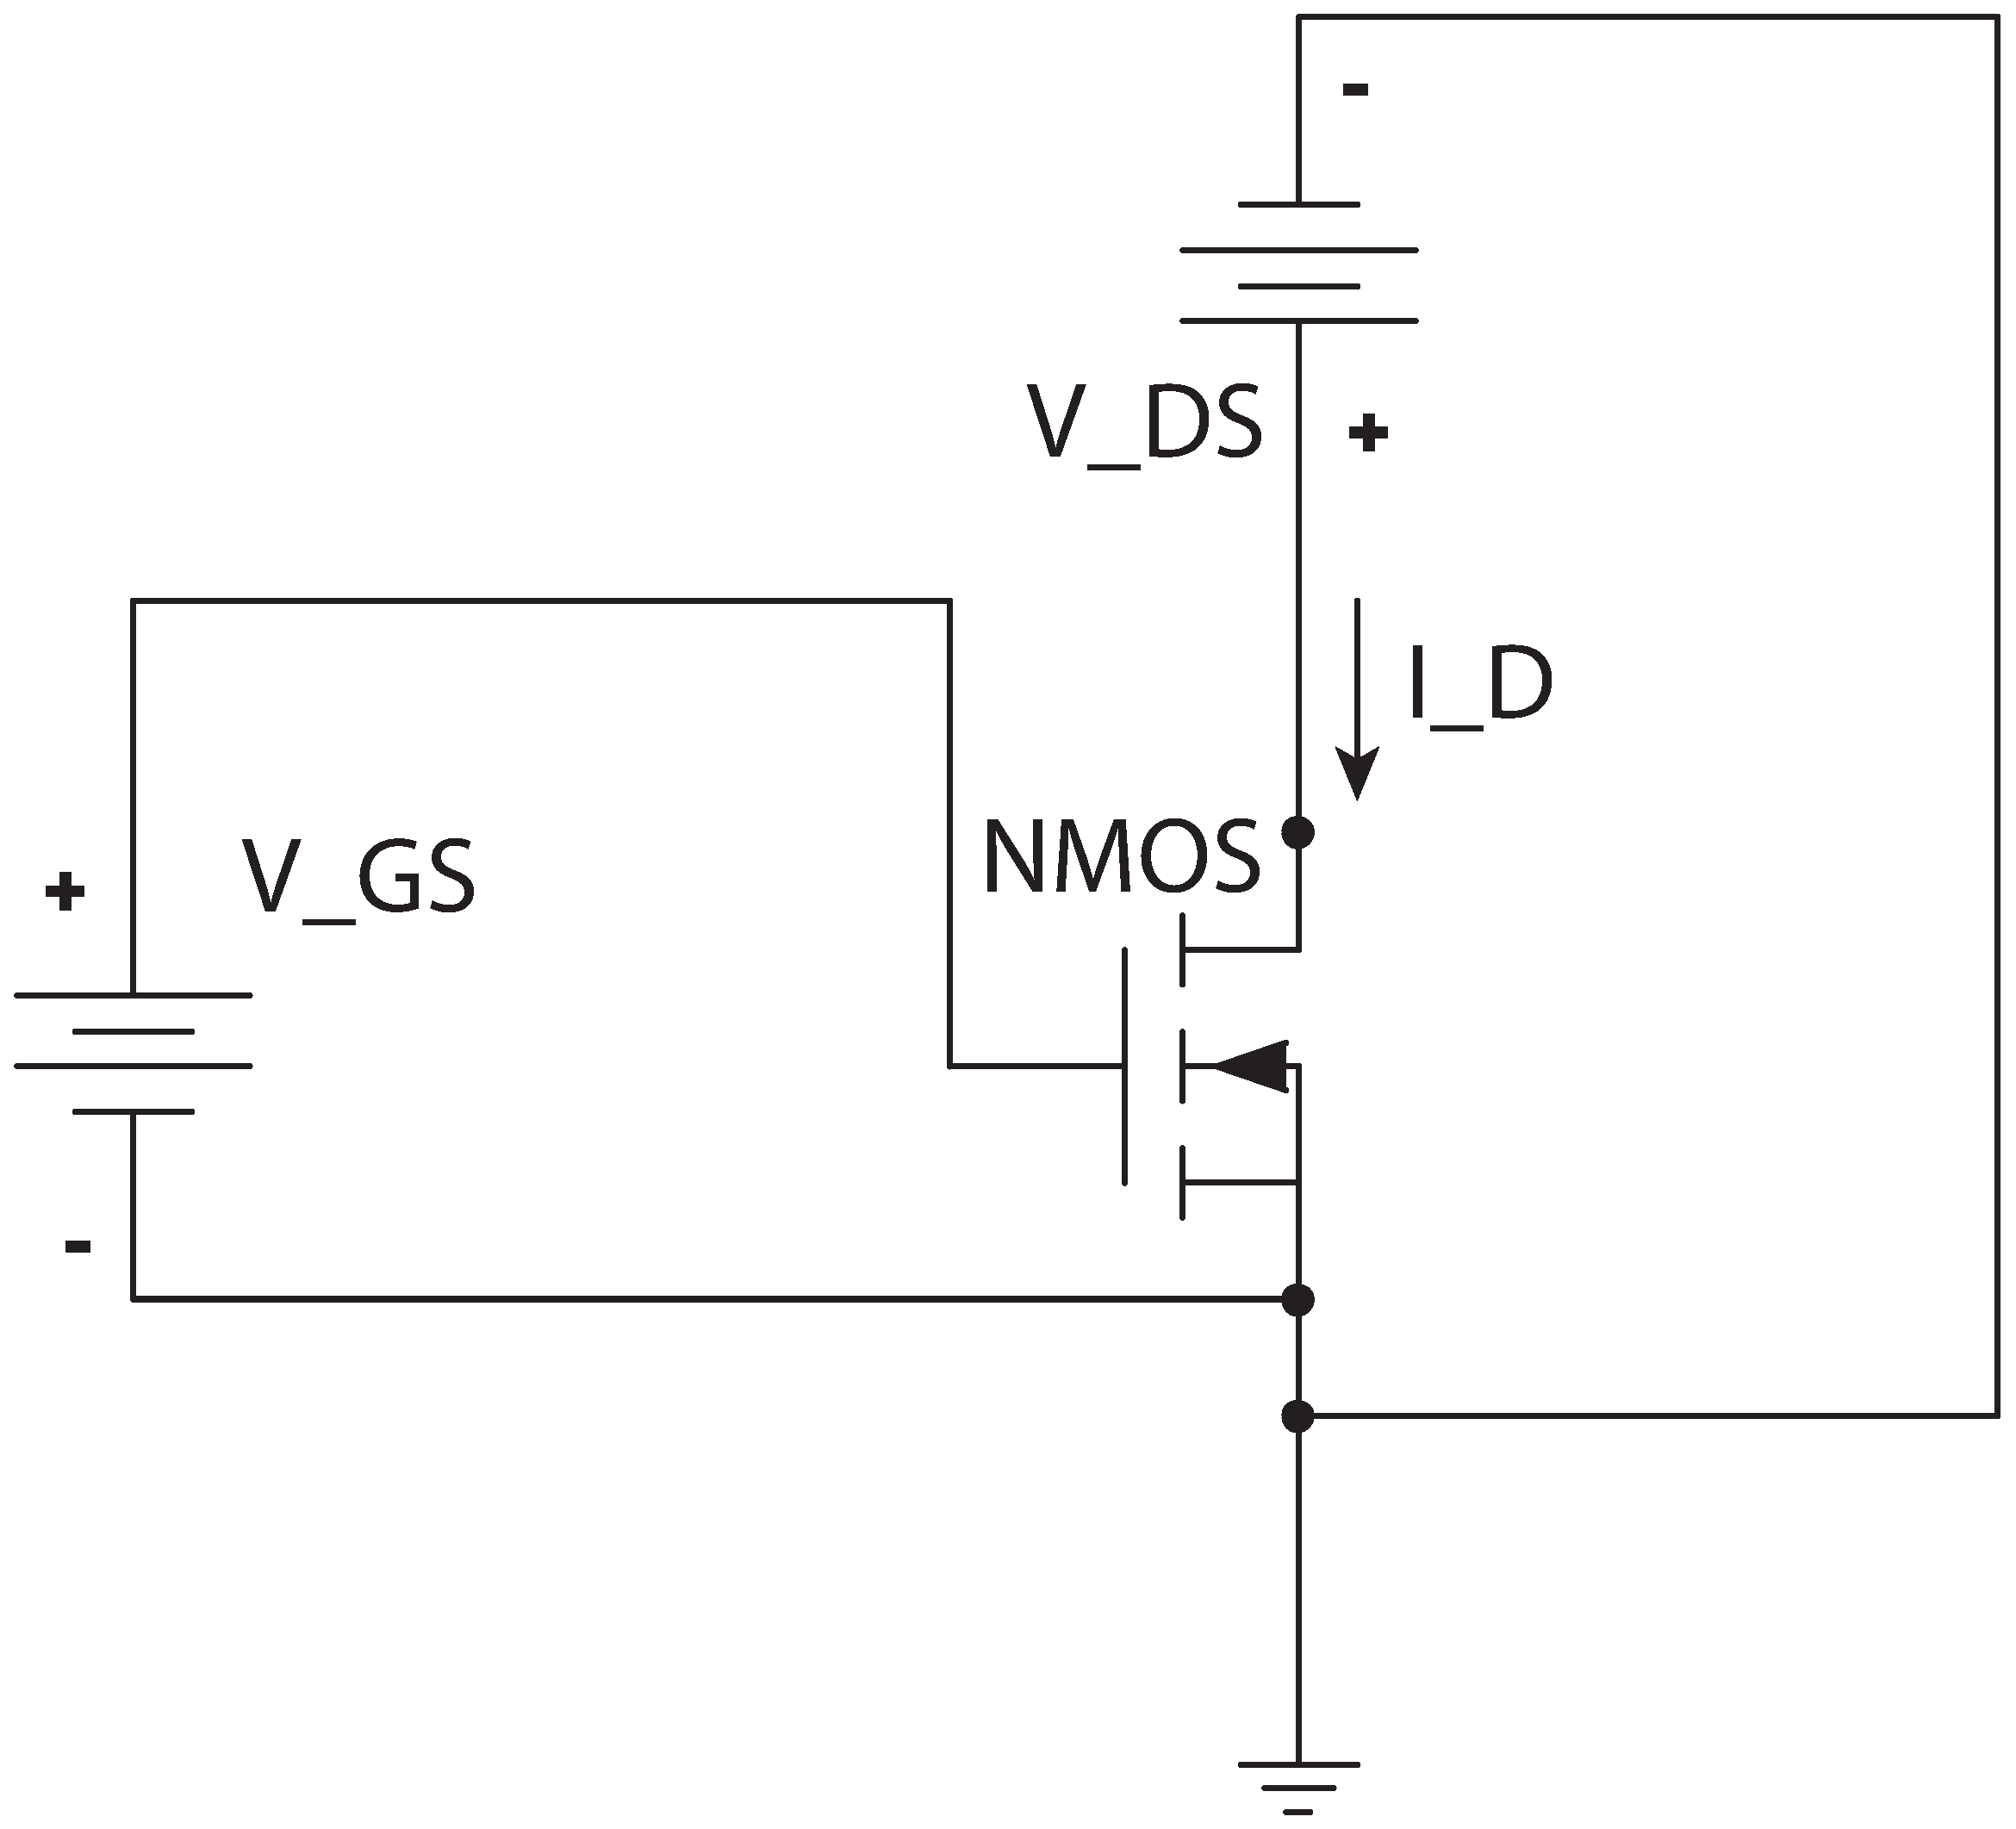
\includegraphics[width=\textwidth]{resources/NMOS_circuit}
		\caption{Het circuit gebruikt om te simlueren.}
		\label{fig:circuit}
\end{figure}


\section{Resultaten}
Het resultaat van de simulatie van ons circuit ziet er als volgt uit.
\begin{figure}[H]
\centering
		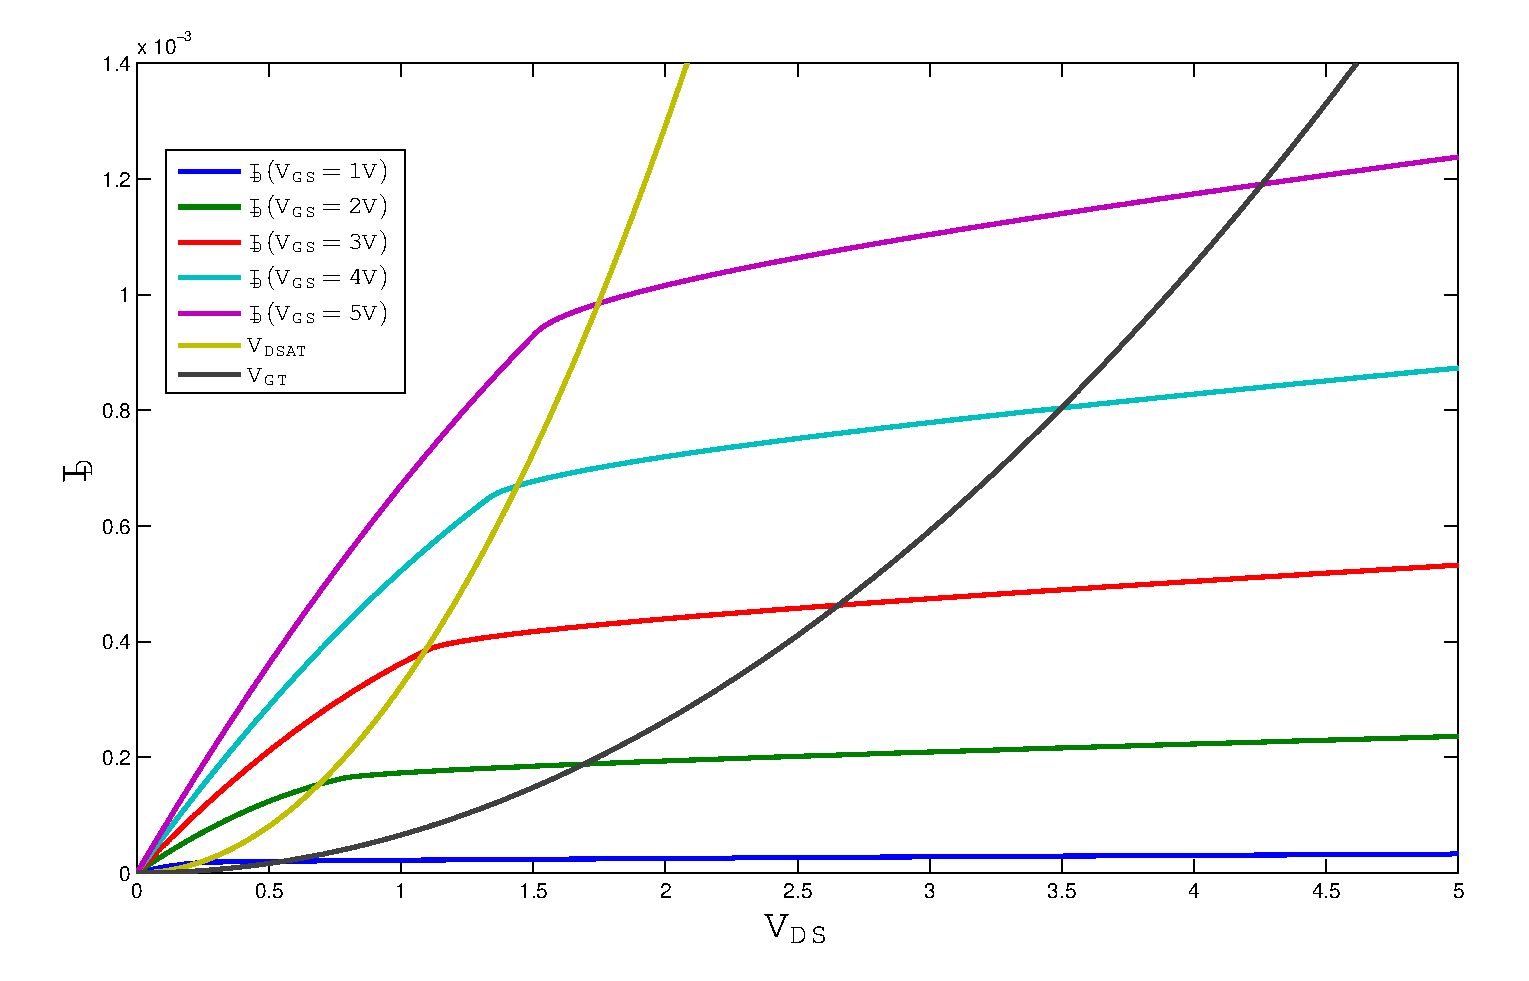
\includegraphics[width=\textwidth]{resources/Id}
		\caption{Het resultaat van de simulatie.}
		\label{fig:Id}
\end{figure}
De verschillende $I_{D}$ lijnen komen rechtstreeks van het circuit. Om de andere 2 lijnen ($V_{DSAT}$ en $V_{GT}$) te kunnen plotten hebben we echter andere dingen moeten doen. Zo hebben we om de $V_{DSAT}$ te kunnen plotten allereerst de tweede afgeleide van de $I_{D}$ grafieken geplot (zie figuur \ref{fig:Id}) en vervolgens daarvan de minima genomen. 
Om vervolgens $V_{GT}$ te kunnen plotten, hebben we de formule: 
\begin{equation}
V_{GS} - V_{T} = V_{DS} 
\end{equation} gebruikt.
\newline $V_{T}$ vonden we door de formule: 
\begin{equation}
V_{T} = V_{T0} + \gamma (\sqrt {2 \phi F + |V_{SB}|} - \sqrt{ 2 \phi F} ) 
\end{equation} in te vullen. $V_{SB}$ = 0, waardoor $V_{T}$  gelijk is aan $V_{T0}$. $V_{T0}$ heeft een vaste waarde van 0.43V. Hiermee konden we dus heel makkeijk vijf verschillende punten vinden en door deze met elkaar te verbinden vonden we de $V_{GT}$ grafiek. 
\newline Aan de van de simulatieresultaten kunnen we nu de werkgebieden aangeven.
\begin{itemize}
	\item Het lineaire gebied is het gebied dat links ligt ten opzichte van de $V_{DSAT}$ lijn;
	\item Het snelheisverzadigingsgebied is het gebied ligt rechts ten opzichte van de $V_{DSAT}$ lijn;
	\item Het 'gewone' verzadigingsgebied zou normaal het gebied zijn dat links ligt ten opzichte van de $V_{GT}$ lijn, maar daar is hier geen sprake van, omdat er al snelheidsverzadiging plaatsvindt.
\end{itemize}

\begin{figure}[H]
\centering
		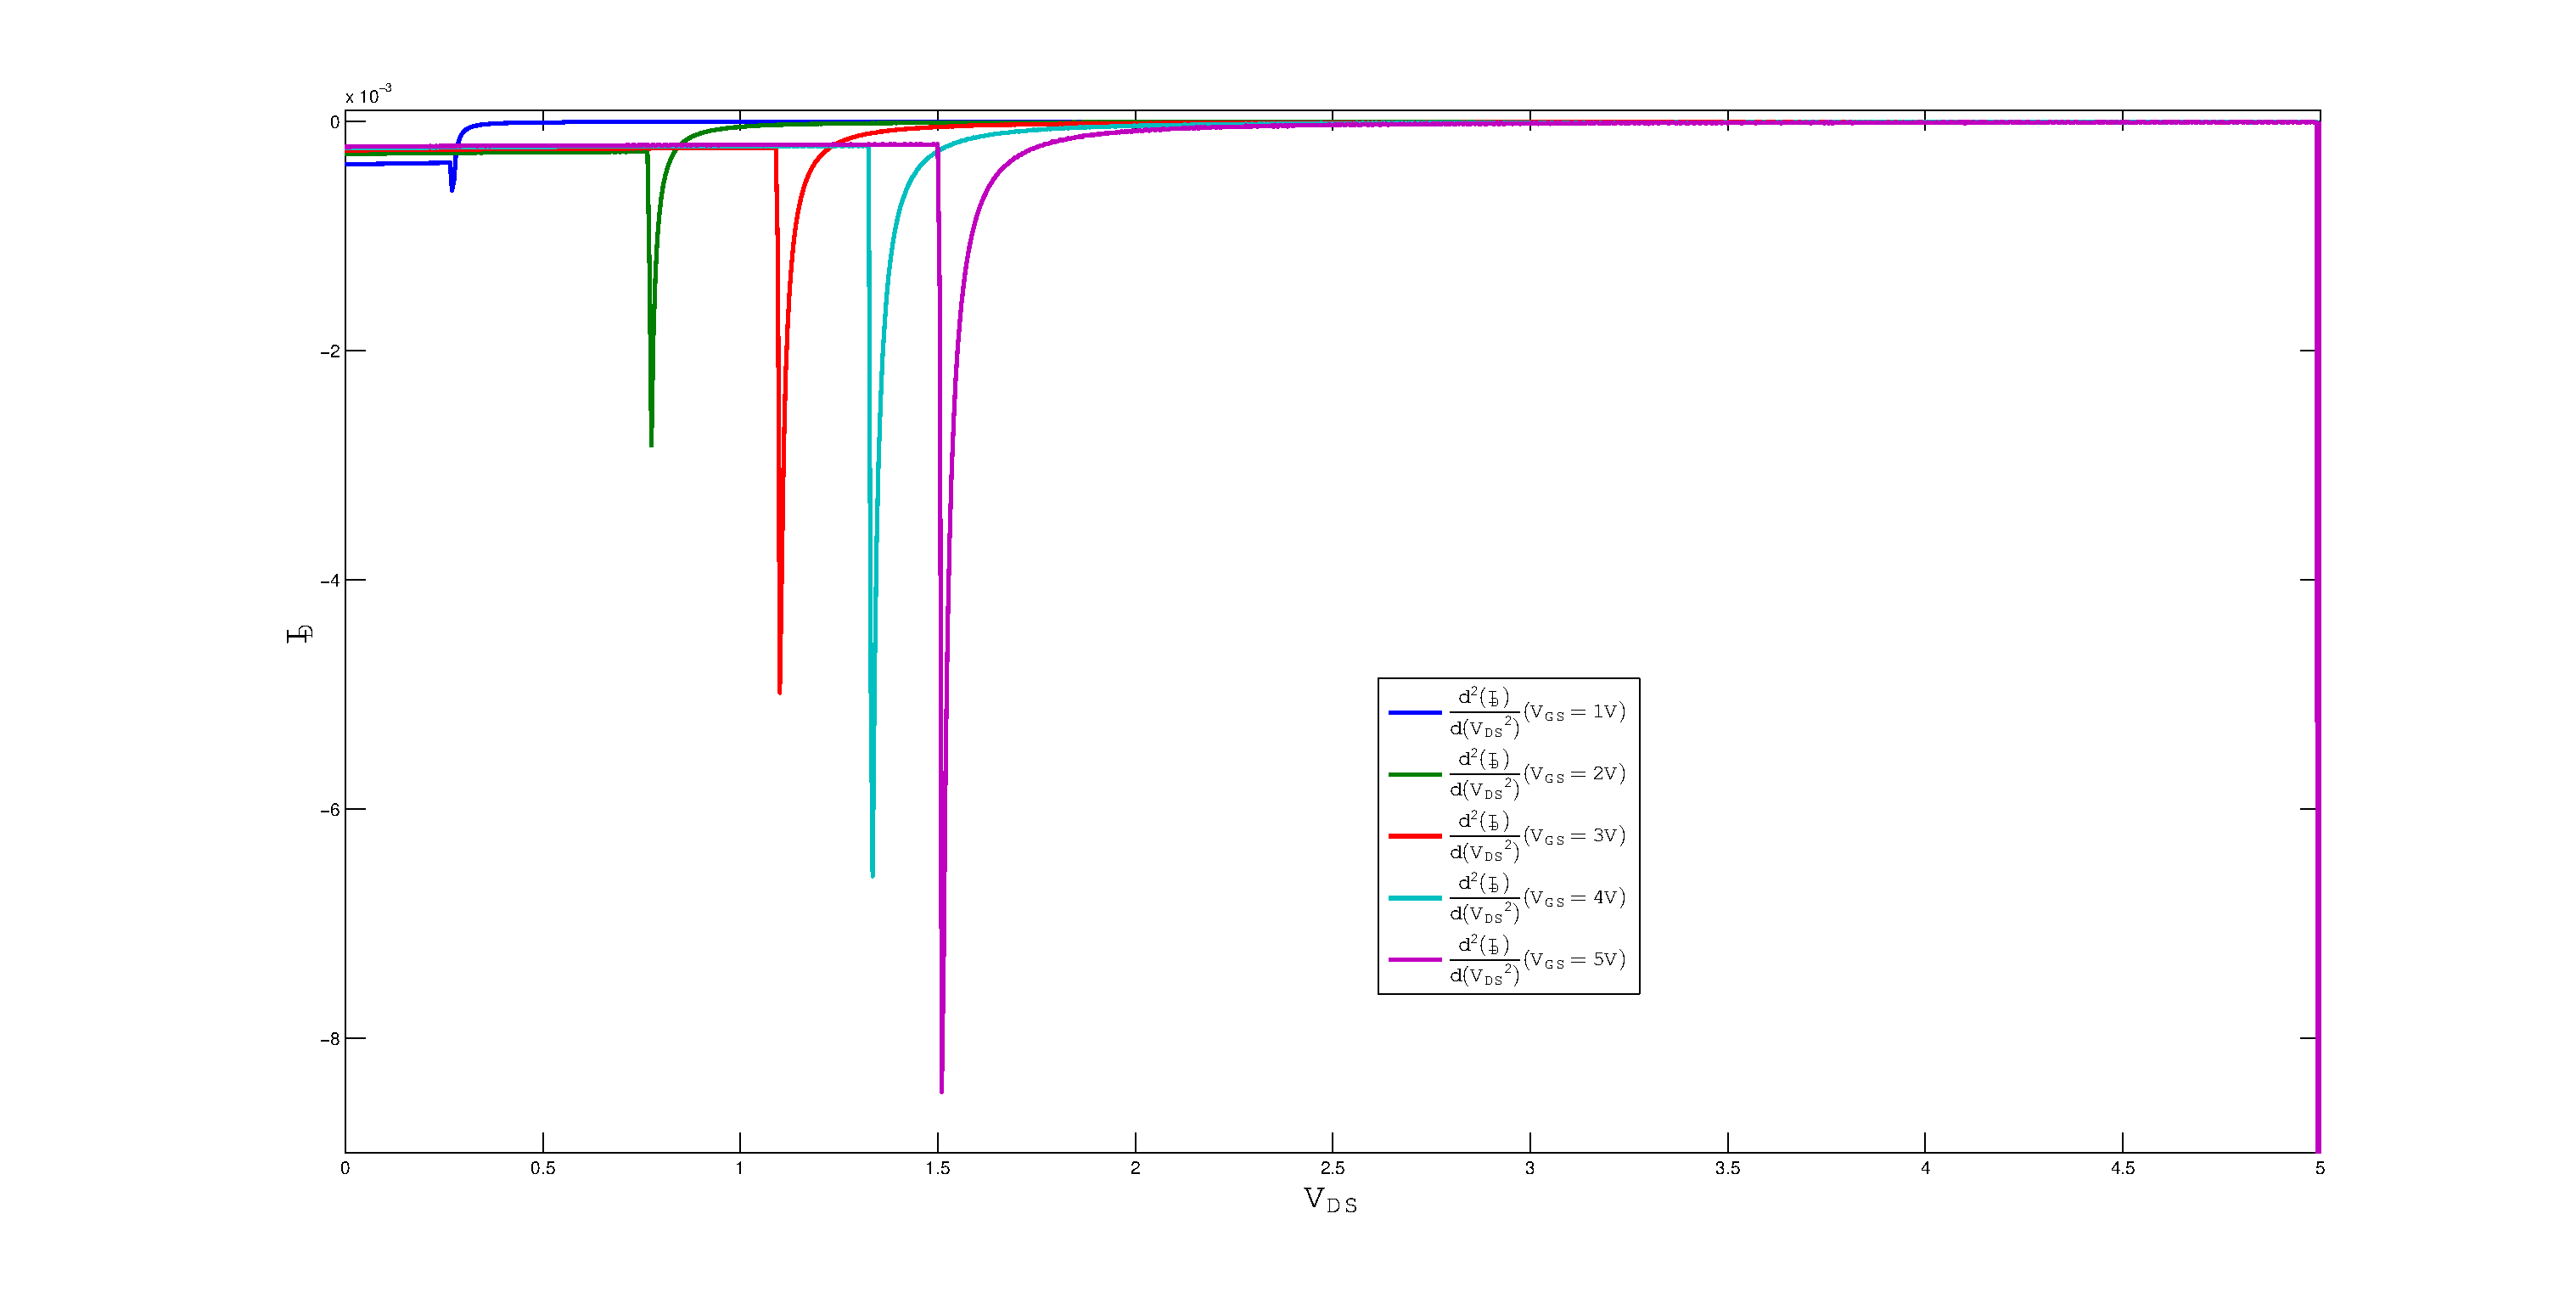
\includegraphics[width=\textwidth]{resources/Id_Vds_2nd_div}
		\caption{De tweede afgeleide van de originele grafiek.}
		\label{fig:Id-2nd-div}
\end{figure}


\section{Discussie}
Zoals te lezen is in de vorige paragraaf konden we goed de verschillende werkgebieden aflezen uit de grafiek. De verkregen resultaten zijn zoals we vooraf al verwacht hadden. Wanneer we de opdracht nog een keer zouden moeten doen, dan zouden we dit op dezelfde manier doen, omdat we geen grote fouten of onnauwkeurigheden hebben geconstateerd. 

\section{Conclusie}
Uit onze verkregen resultaten kunnen we de volgende conclusie trekken: 

\section{Bibliografie}
\printbibliography
